\chapter{Grundlagen}
Dieses Kapitel erläutert die grundlegenden Begriffe und Konzepte, die zum 
Verständnis dieser Bachelorarbeit notwendig sind. 
Dabei wird der Technologie-Stack aufsteigend beschrieben.
Als Fundament dient die Container Technologie Docker.
Orchestriert wird diese durch die Containerplattform Kubernetes.
Abschließend folgt ein Abschnitt zu Microservices.

%TEXT!!!!

\section{Docker} \label{Docker}

In diesem Abschnitt wird die Technologie Docker näher erläutert und
nicht das Unternehmen Docker, Inc. ,welches für die maßgebliche Entwicklung dessen verantwortlich ist \cite[S.11]{dockerdeep}.
Es folgt eine aufsteigende Erklärung der Architektur hin zum Aufbau eines Containers.

%\subsection{Terminologie}
%\begin{itemize}
%    \item \textbf{Container}: Isolierter Prozess mit einer laufenden Anwendung.
%    \item \textbf{Volumes}: Persistente Daten eines Containers.
%    \item \textbf{Image}: Einheit mit ausführbaren Code, Abhängigkeiten und Betriebssystem. Aufgeteilt in mehreren Schichten.
%    \item \textbf{Dockerfile}: Textdatei zum erstellen eines Docker-Images.    
%\end{itemize}

\subsection{Architektur}
Die Docker-Technologie ist in der Programmiersprache GO geschrieben und nutzt Funktionalitäten des
Linux-Kernels, wie cgroups und namespaces.
Namespaces ermöglichen die Isolation von Prozessen in sogenannte Container, welche unabhängig voneinander arbeiten \cite{dockergetstarted}.
Diese beeinhalten alle nötigen Abhängigkeiten zur Ausführung der vordefinierten Anwendungen.
Container gewinnen dadurch an Portabilität,
sodass sie auf allen Infrastrukturen mit Docker-Laufzeit bereitgestellt werden können.
Die Laufzeit setzt sich aus \glqq runc\grqq{} einer low-level-Laufzeit und \glqq containerd\grqq{} einer higher-level-Laufzeit zusammen (vgl. Abbildung~\ref{fig:dockerarch}).
Runc dient als Schnittstelle zum Betriebssystem und startet und stoppt Container.
Containerd verwaltet die Lebenszyklen eines Containers, das Ziehen von Images, das Erstellen von Netzwerken und die Verwaltung von runc.
Die allgemeine Aufgabe des Docker-Daemons ist es, eine vereinfachte Schnittstelle für die Abstraktion
der darunterliegenden Schicht zu gewährleisten, wie zum Beispiel dem Verwalten von Images, Volumes und Netzwerken \cite[S.12]{dockerdeep}.
Auf die Orchestrierung mit Swarm wird nicht weiter eingeganen, da sie zum Verständnis nicht nötig ist.

\begin{figure}
    \centering
    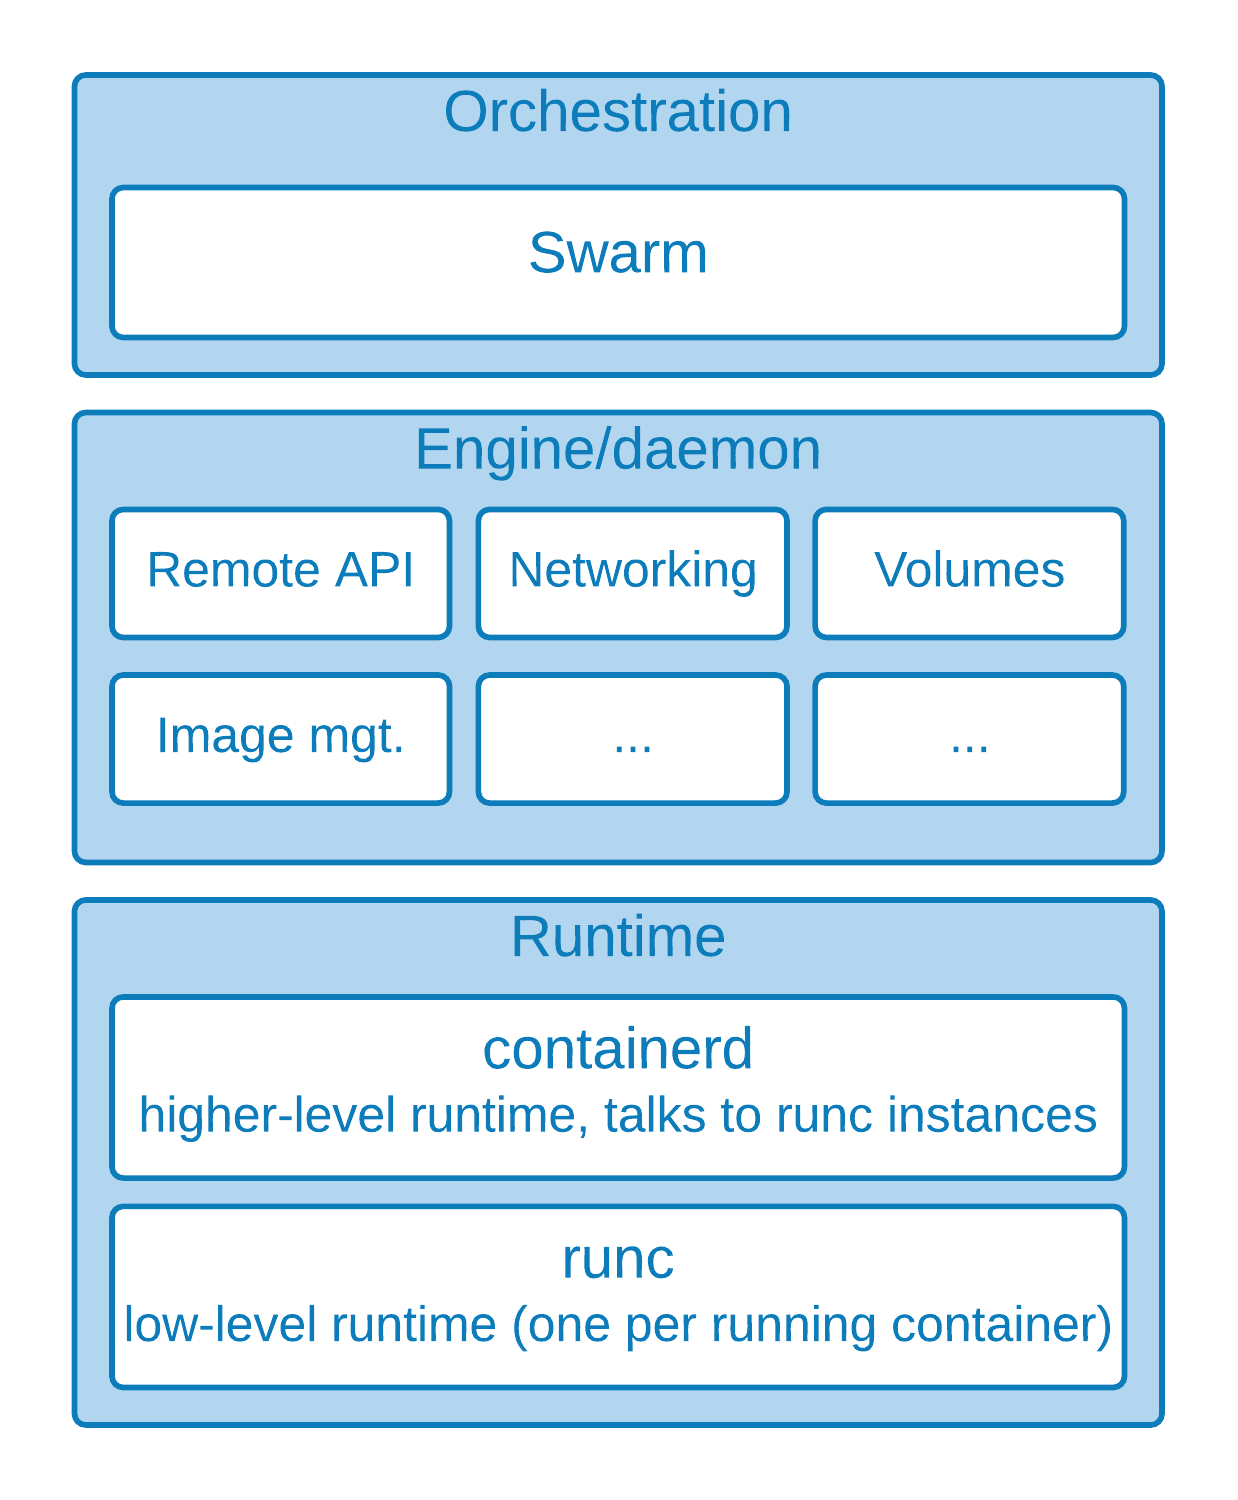
\includegraphics[width=0.5\columnwidth]{images/DockerArch.png}
    \caption{Docker Architektur in Anlehnung an \protect\cite[S.11]{dockerdeep}}
    \label{fig:dockerarch}
\end{figure}

\subsection{Images und Container}
Ein Docker-Image ist ein Objekt, das alle Abhängigkeiten, wie Quellcode, Bibliotheken und Betriebssystemfunktionen für eine Anwendung beeinhaltet. 

\subsubsection{Registrys}
Das beziehen von Images erfolgt über sogenannte \glqq Image Registries\grqq{}.
Bei Docker ist dies standardmäßig \url{https://hub.docker.com} und das eigene lokale Registry. 
Es ist auch möglich, eigene zu hosten oder diejenigen von Drittanbietern zu nutzen.

\subsubsection{Schichten}
Docker Images bestehen aus mehreren Schichten, jede davon abhängig von der Schicht unter ihr und
erkennbar durch IDs in Form von \acs{sha}256-Hashes (vgl. Abbildung~\ref{fig:dockerlayer}).
Docker kann dadurch beim Bauen oder Updaten von neuen Images vorhandene Schichten erneut verwenden. 
Die feste Reihenfolge ermöglicht eine ressourceneffiziente Verwaltung von Builds,
indem man oft wechselnde Schichten oben platziert. 
Die Leistung beim Erstellen und Zusammenführen von Schichtem hängt vom Dateisystem des Hostsystems ab.
Eine Schicht kann aus mehreren Dateien bestehen
und einzelne Dateien aus der unterliegenden Schicht mit einer neuen ersetzen.

\begin{figure}
    \centering
    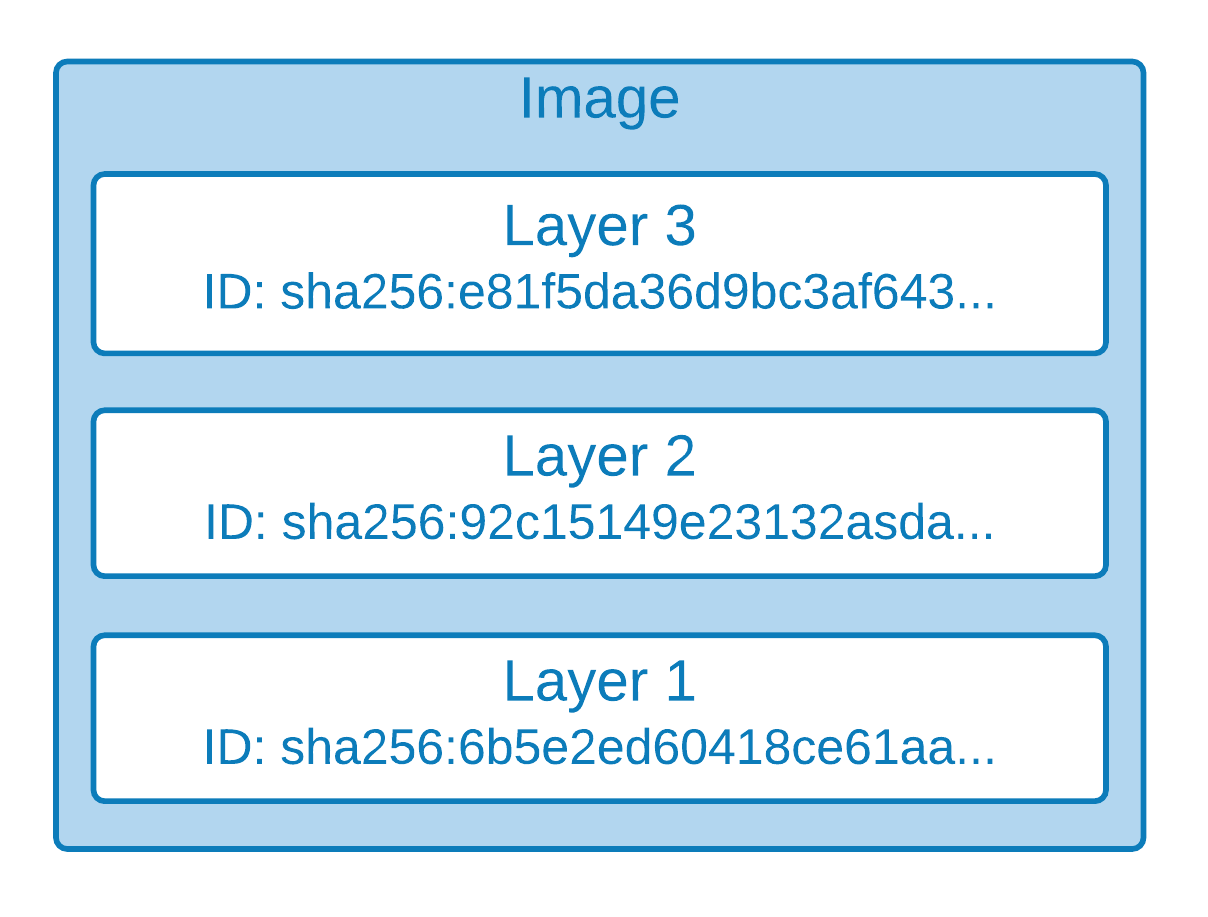
\includegraphics[width=0.5\columnwidth]{images/Image-Layer.png}
    \caption{Image Layers in Anlehnung an \protect\cite[S.61]{dockerdeep}}
    \label{fig:dockerlayer}
\end{figure}

%copy-on-write (CoW) strategy???

%nicht alle dockerfile anweisungen erstellen layer ENV expose usw.
Das Starten eines Containers fügt auf die bereits bestehenden Schichten einen \glqq Thin R/W layer\grqq{} 
- \glqq Container layer\grqq{} genannt - hinzu. Dieser gewährt Schreib- und Leserechte während der Laufzeit des Prozesses. 
Jeder dieser Container hat somit einen individuellen Zustand, der unähnlich vom abstammendem Image ist.
Bei Löschung des Containers verschwindet auch die dazugewonnene Schicht.
Das Entfernen eines Images ist durch die Konzeption des Schichtensystem erst möglich, wenn alle darauf
basierenden Container gelöscht sind \cite{dockerstoragedriver}.

\subsubsection{Dockerfile}
Zur Erstellung eines Docker-Images wird ein Dockerfile benötigt. Dies beeinhaltet alle Anweisungen
zum Aufbau der einzelnen Schichten. 
Diese Aufrufe erstellen die Schichten eines Images \cite{dockerbestpracticedockerfile}.
\begin{itemize}
    \item \textbf{FROM} Erstellen einer Schicht auf Basis eines base-images. 
    \item \textbf{COPY} Hinzufügen von Dateien aus dem aktuellen Arbeitsverzeichnis. 
    \item \textbf{RUN} Bauen der Anwendung mit make. 
\end{itemize}
Diese hingegen fügen nur Metadaten hinzu \cite{dockerbestpracticedockerfile}.
\begin{itemize}
    \item \textbf{EXPOSE} informiert Docker, an welchem Port der Container innerhalb seines Netzwerks lauscht.
    \item \textbf{ENTRYPOINT} ermöglicht es, einen Container als ausführbare Datei zu starten.
    \item \textbf{CMD} Befehl beim Ausführen des Containers.
\end{itemize}


\subsection{Containervirtualisierung}
Aus dem Wissen des letzten Abschnitts lässt sich schlussfolgern, dass
ein Container eine laufende Instanz eines Images ist.
Vergleichbar ist dieses Konzept mit dem einer \acs{vm}.
Denn Images ermöglichen ähnlich wie \acs{vm}-Templates die Erstellung von mehreren Instanzen durch eine Vorkonfiguration.
Mit dem Unterschied, dass die Einrichtung von \acs{vm}s arbeitsintensiver ist und weitaus mehr Ressourcen
beansprucht, da sie ein ganzes Betriebssystem ausführt \cite{hypervisorcontainer}. Containertechnologien bauen hingegen nur auf 
bestimmte Funktionalitäten des Kernels auf und sparen damit an Rechenleistung (vgl. Abbildung~\ref{fig:containervm}).

Durch die Vorteile eines geteilten Kernels und dessen Betriebssystemabhängigkeiten,
erzielen Virtualisierungen basierend auf Containern eine höhere Anzahl an 
virtuellen Instanzen. Images beanspruchen weniger Speicherplatz als hypervisor-basierende Ansätze \cite{hypervisorcontainer}.

\begin{figure}
    \centering
    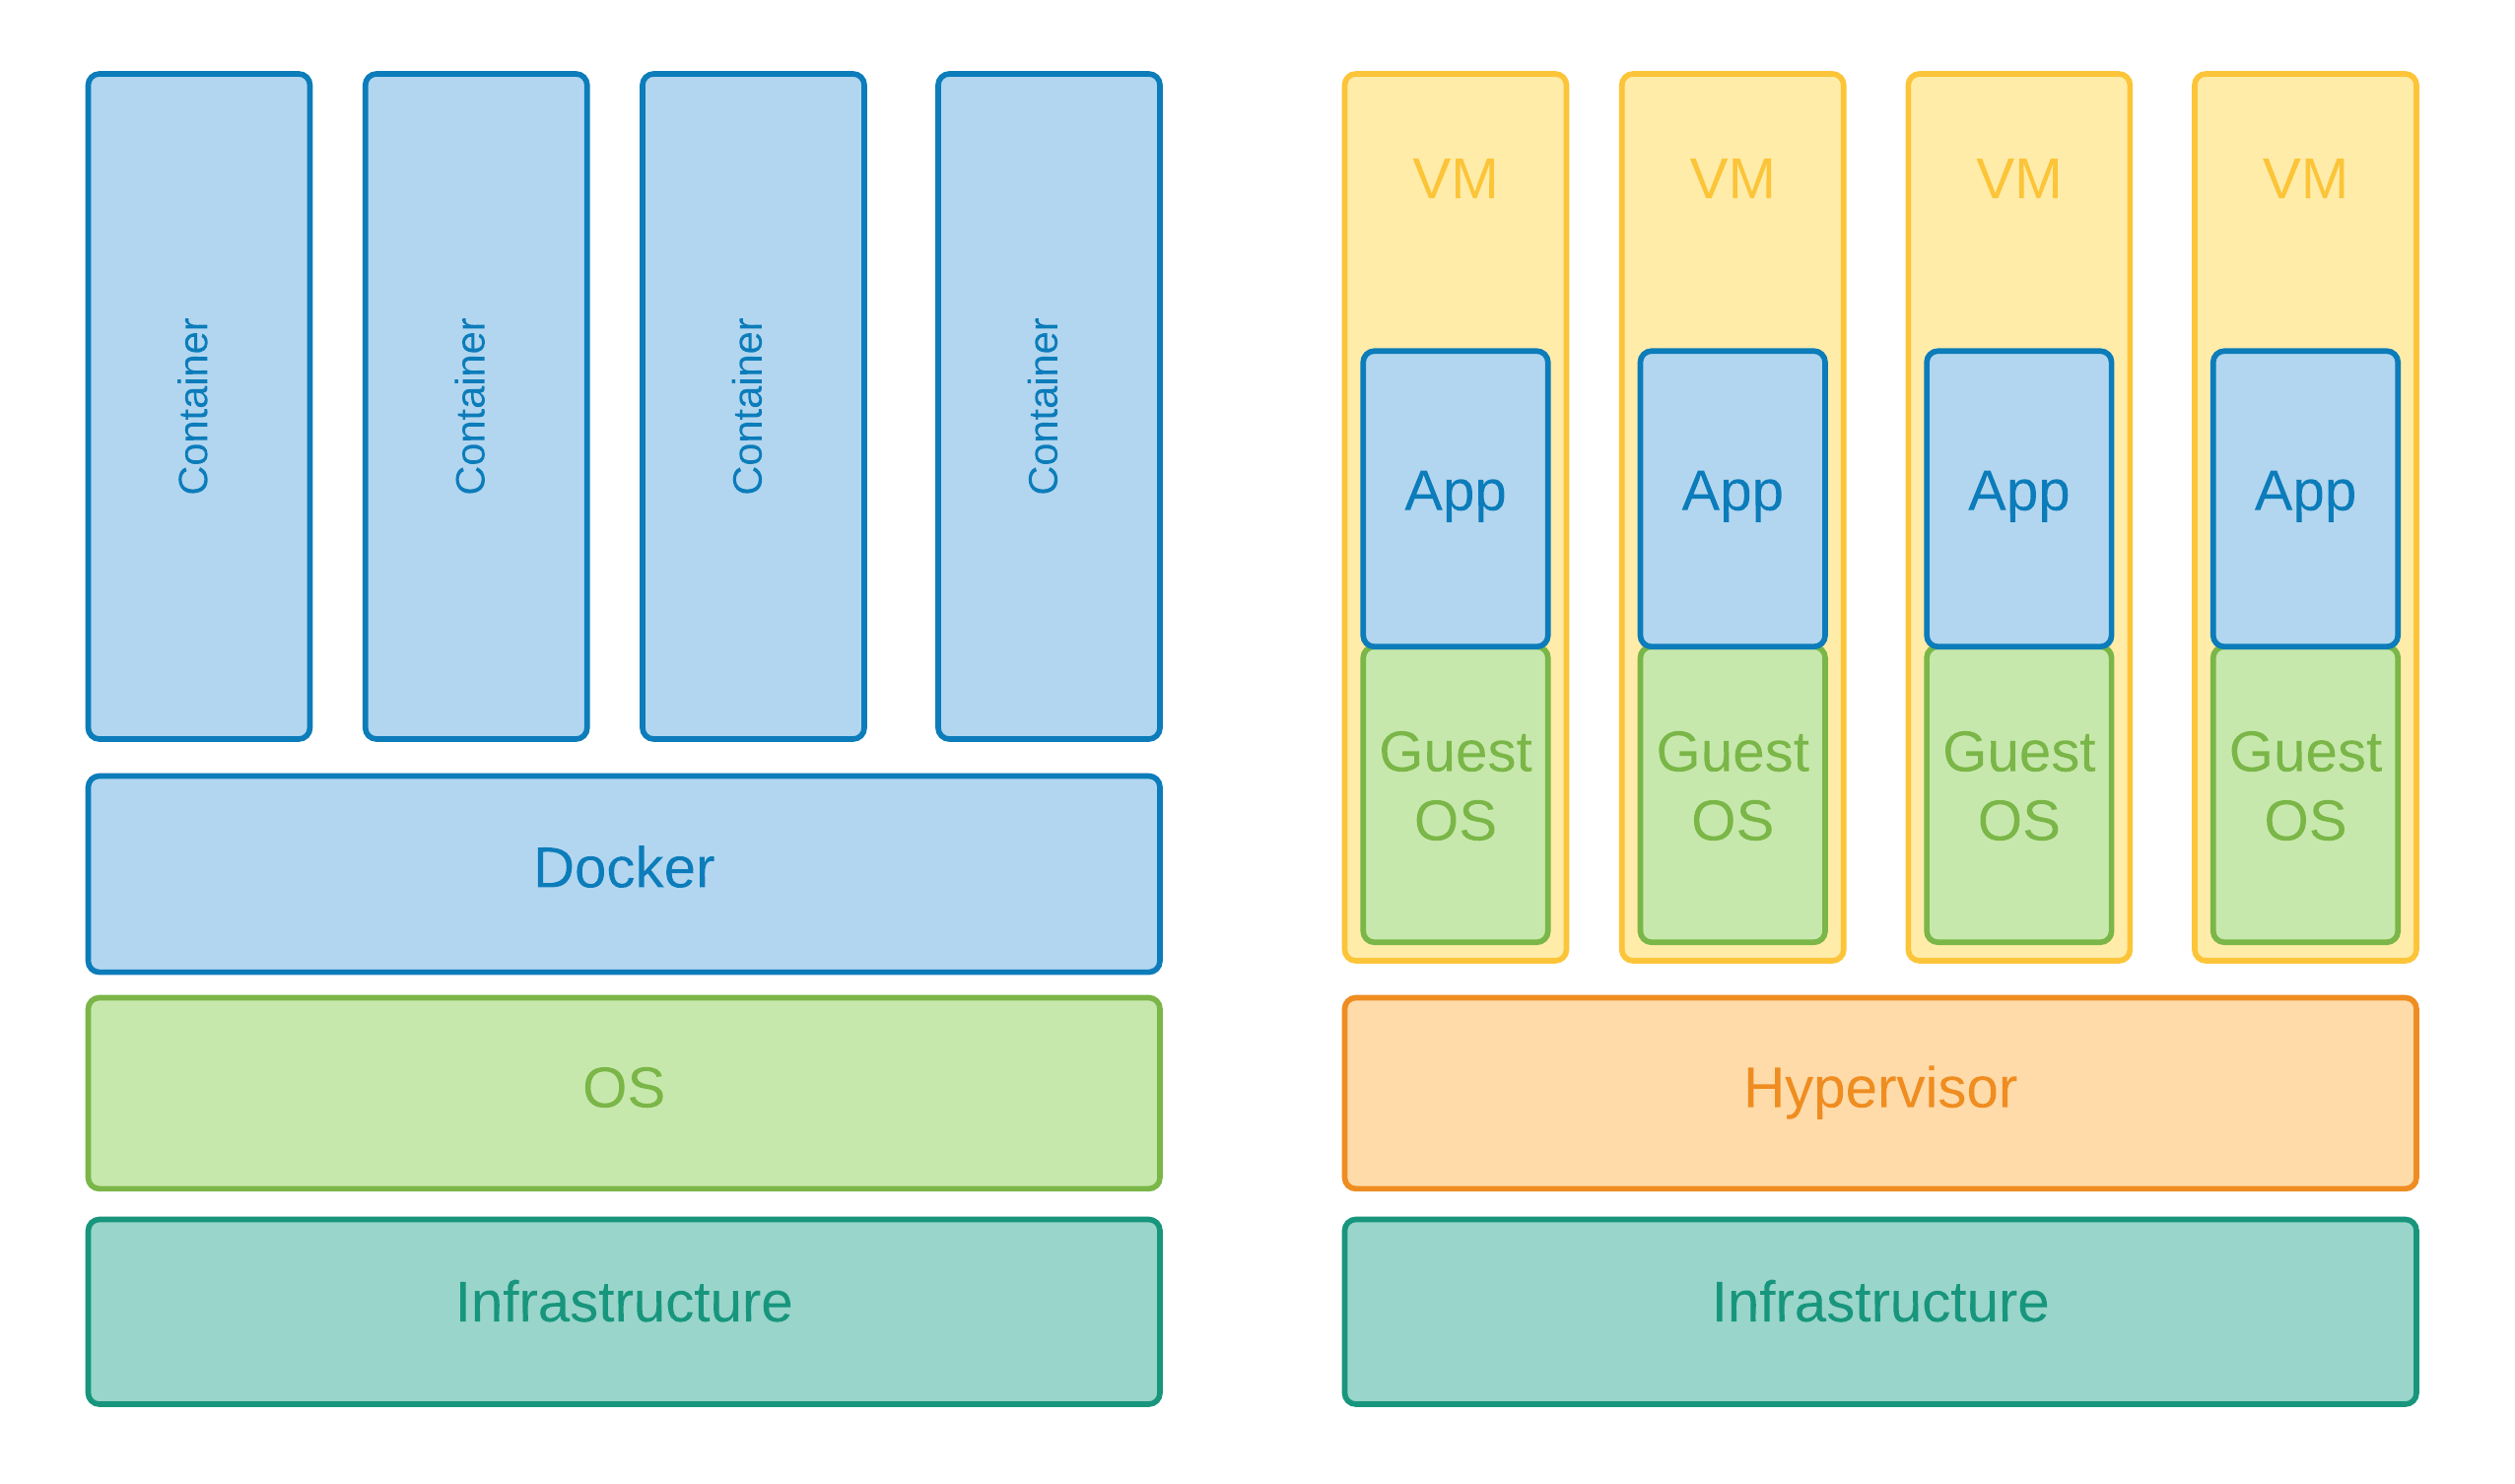
\includegraphics[width=1.0\columnwidth]{images/Container-VM.png}
    \caption{Virtualisierungsmöglichkeiten angelehnt an \protect\cite{containervsvm}.}
    \label{fig:containervm}
\end{figure}

Die Einsparung von Ressourcen und dem einfachen Bereitstellen auf Hostsystemen
prädestinieren containerisierte Anwendungen für die Verwendung von Microservices
auf Containerplattformen, wie Kubernetes.


\section{Kubernetes}
\begin{quote}
  \glqq Der Name Kubernetes stammt aus dem Griechischen, bedeutet Steuermann oder Pilot, [...]
K8s ist eine Abkürzung, die durch Ersetzen der 8 Buchstaben \dq ubernete\dq{} mit \dq 8\dq{} abgeleitet wird\grqq{} \cite{kubernetes}.
\end{quote}


Dieser Abschnitt befasst sich zunächst mit den einzelnen Komponenten der Kubernetes-Architektur.
Hinleitend werden spezielle Themen wie k3s, Hybrid Cloud und Rancher näher erläutert.
Kubernetes ermöglicht die Orchestrierung von containerisierten Arbeitslasten
und Diensten. Seit 2014 hat Google das Open-Source-Projekt zur Verfügung
gestellt und baut auf 15 Jahre Erfahrungen mit Produktions-Workloads auf \cite{kubernetes}.

\subsection{Cluster}
Die Zusammensetzung der beschriebenen Kubernetes-Komponenten ergeben ein Kubernetes-Cluster (vgl. Abbildung~\ref{fig:cluster}).


\begin{figure}
    \centering
    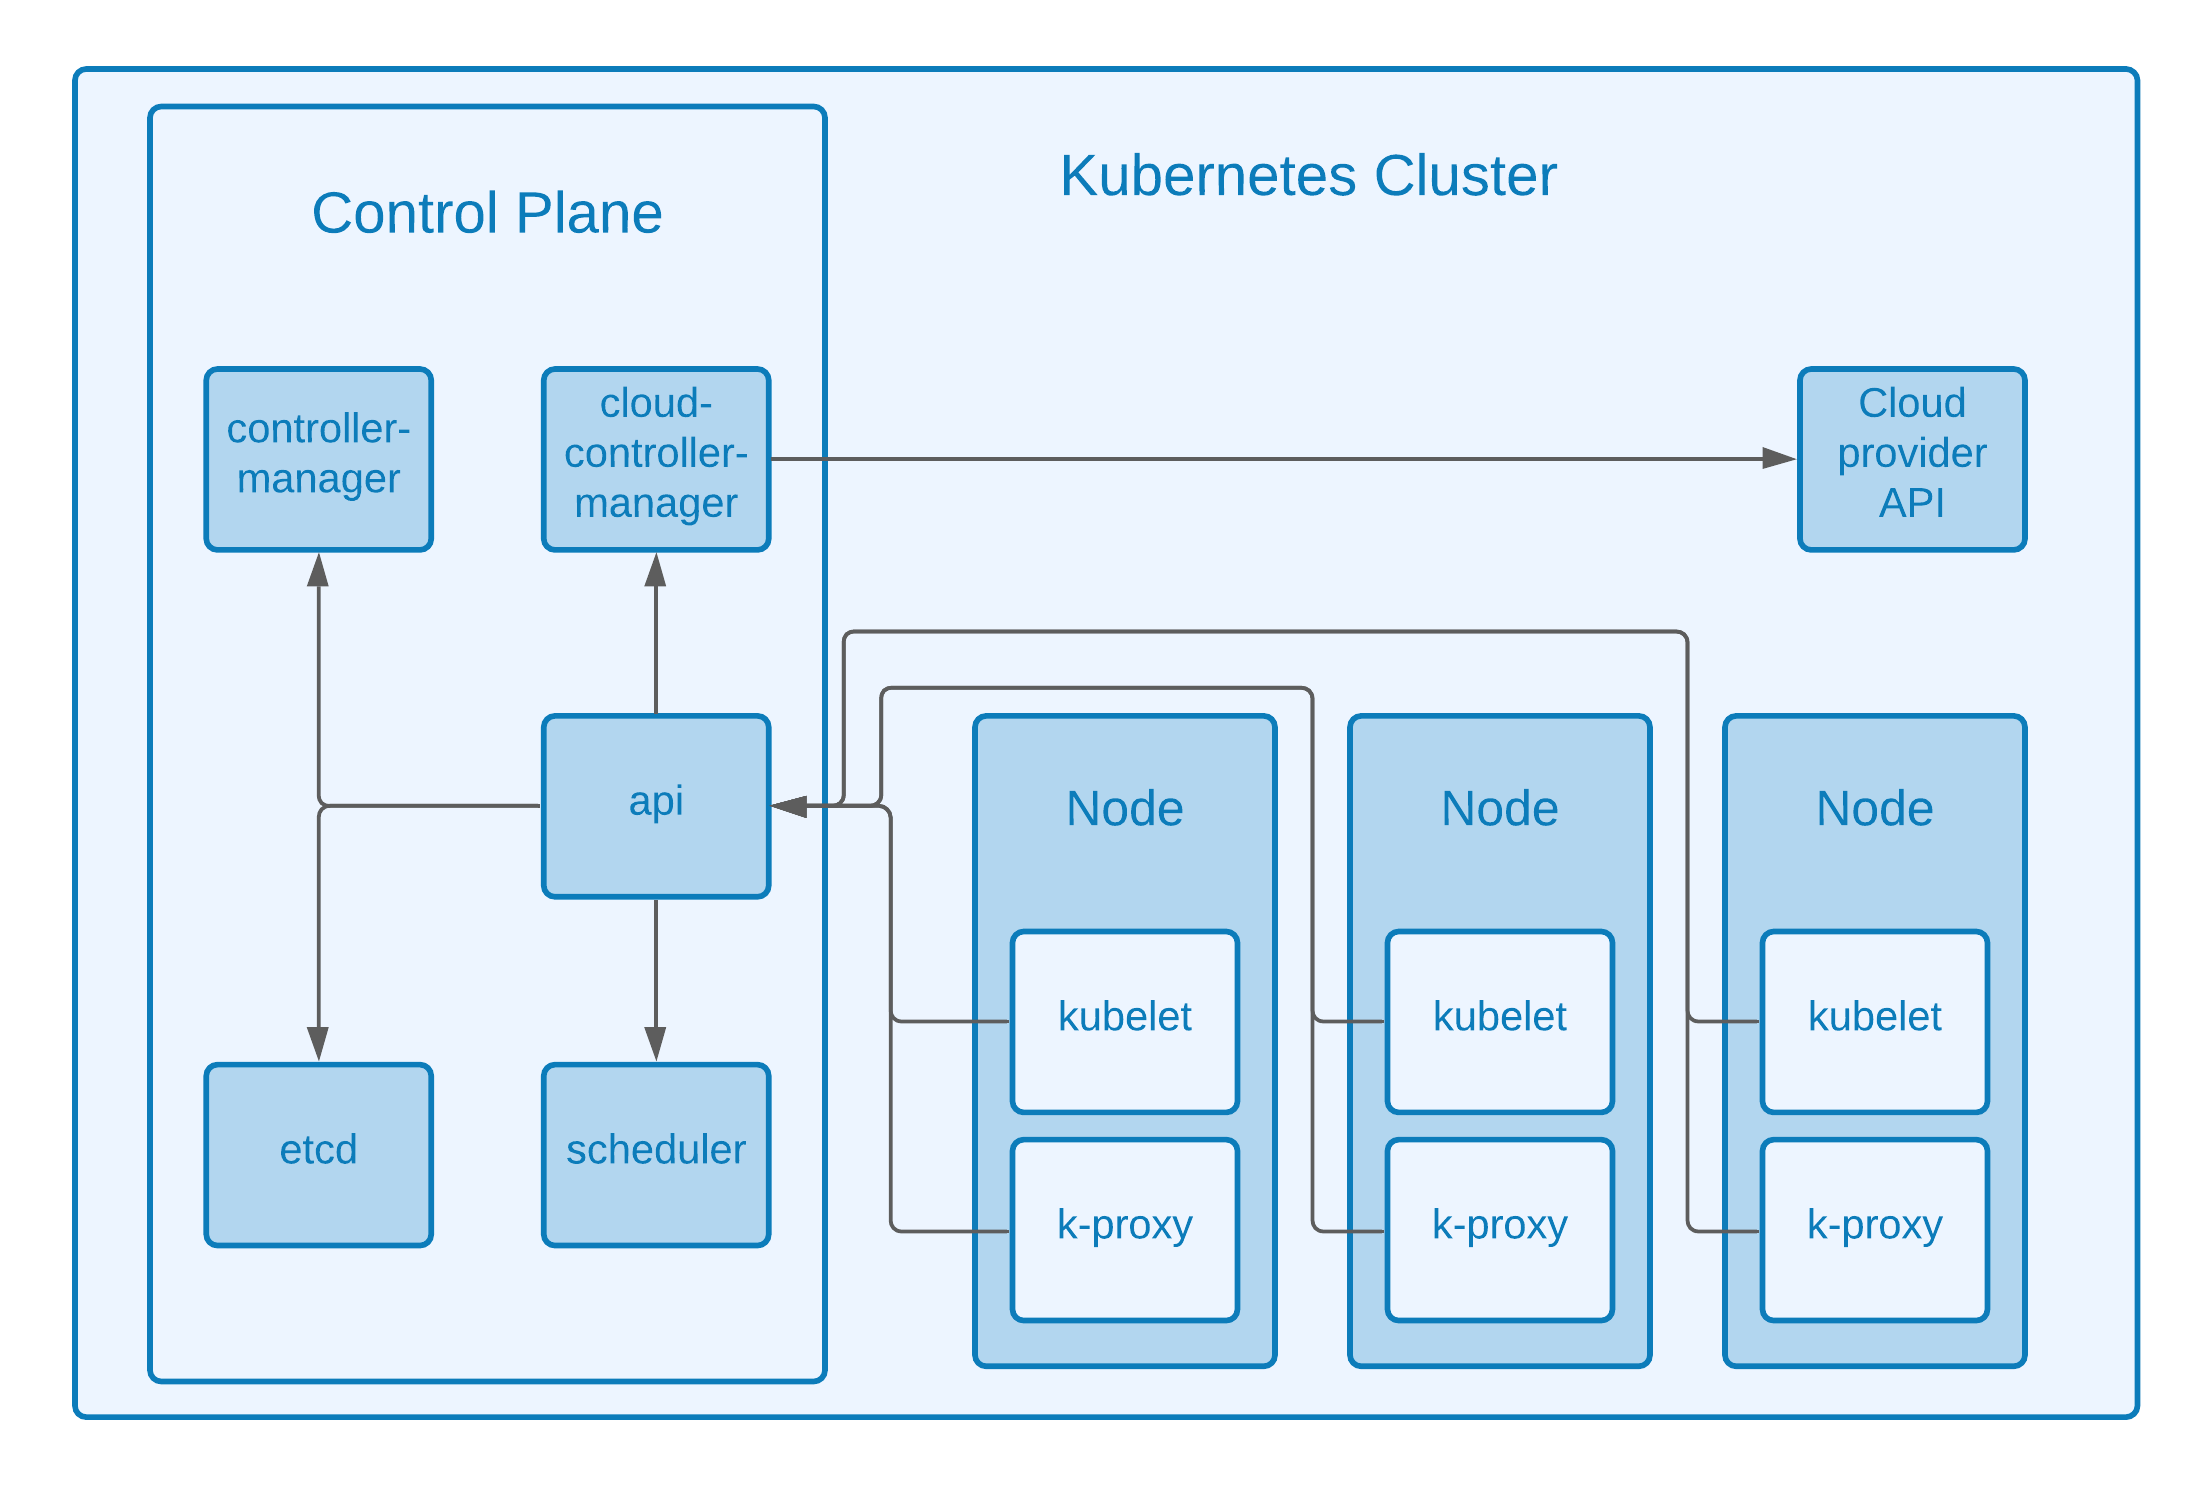
\includegraphics[width=1.0\columnwidth]{images/KubernetesKomponenten.png}
    \caption{Komponenten eines Kubernetes Cluster in Anlehnung an \cite{kuberneteskomponenten}.}
    \label{fig:cluster}
\end{figure}

\subsubsection{Control Plane}
Control Planes\footnote{Seit Kubernetes v1.20, ist Control Plane die korrekte Bezeichnung für die Master Node \cite{Kuberneteschangemaster}} sind für die Steuerungsebene des Clusters zuständig.
Dabei entscheidet und reagiert dieser auf globaler Ebene auf eintreffende Clustereignisse.
Die Kubernetes-Dokumentation beschreibt diese Komponenten wie folgt \cite{kuberneteskomponenten}:

\begin{itemize}
  \item \textbf{\acs{api}-Server}: Der \acs{api}-Server ist \acs{rest}-konform und bietet eine Schnittstelle zu Diensten
  inner- und außerhalb der Control-Plane.
  \item \textbf{etcd}: etcd ist der primäre Datenspeicher von Kubernetes und sichert alle Zustände eines Clusters.
  \item \textbf{Scheduler}: Der Scheduler ist zuständig für die Verteilung und Ausführung von Pods auf Nodes.
  \item \textbf{Controller Manager}: Der Controller Manager reagiert auf Ausfälle von Nodes, stellt die korrekte Anzahl von Replikationen eines Pods sicher und verbindet Services miteinander.
\end{itemize}

\subsubsection{Node}
Eine Node\footnote{Um den Sprachfluss zu wahren wird der englische Begriff Node, als Kubernetes-Ressourcenobjekt nicht übersetzt. 
Die Übersetzung Knoten findet lediglich als Hardwareinstanz statt.} 
ist eine Hardware-Einheit, die je nach Kubernetes-Einrichtung eine \acs{vm}, eine physische Maschine oder 
eine Instanz in einer privaten oder öffentlichen Cloud darstellen kann.
Diese umfasst folgende Komponenten \cite{kubernetesnodes}:

\subsubsection{\textit{Container Laufzeit}}
Die Laufzeit wurde bereits in Abschnitt \hyperref[Docker]{2.1} ausführlich besprochen.
Desweiteren ist es erwähnenswert, dass Containerd als Container-Laufzeit von Kubernetes nach Version 1.20 auslaufen wird \cite{kubernetesdocker}.
Dies beeinträchtigt die spätere Implementierung dieser Arbeit jedoch nicht, da k3s Containerd als Standard Laufzeit weiterhin unterstützt.

\subsubsection{\textit{Kubelet}}
Kubelet fungiert als \glqq node agent\grqq{} und registriert die Node mit dem
\acs{api}-Server eines Clusters und stellt dabei sicher, dass Container innerhalb eines Pods
funktionieren.

\subsubsection{\textit{Kube-Proxy}}
Ein Kube-Proxy ist ein Netzwerk Proxy und verwaltet die Netzwerkzugriffe auf Nodes.
Kube-Proxys erlauben die Kommunikation zwischen Pods inner- und außerhalb des Clusters.

\subsection{Pods}
Ein Pod stellt die kleinste Einheit eines Kubernetes-Clusters dar und ist eine Gruppe aus mindestens einem Container.
Pods erlauben Containern die gemeinsame Nutzung von Speicher- und Netzwerkressourcen.

\subsection{Deployment}
Ein Deployment ist ein Ressourcenobjekt, das mit einem Deployment-Controller den gewünschten Zustand einer Anwendung aufrechterhält.
Diese Spezifikationen sind in Form von \acs{yaml}-Dateien definiert (vgl. Quellcode~\ref{lst:deployment}).
Im Folgenden ist eine kurze Aufschlüsselung der einzelnen Instruktionen \cite{kubernetesobjects}.
\begin{itemize}
    \item \textbf{\acs{api}Version}: definiert die einzelnen Workload-\acs{api}-Untergruppen und die Version.
    \item \textbf{kind}: bestimmt das zu erstellende Kubernetes-Objekt.
    \item \textbf{metadata}: definiert einzigartige Bestimmungsmerkmale.
    \item \textbf{spec}: gewünschter Ausgangszustand des Objekts.
\end{itemize}

\begin{lstlisting}[caption={deployment.yaml \cite{kubernetesdeployment} },captionpos=b,label={lst:deployment},language=yaml]
    apiVersion: apps/v1
    kind: Deployment
    metadata:
      name: nginx-deployment
      labels:
        app: nginx
    spec:
      replicas: 3
      selector:
        matchLabels:
          app: nginx
        spec:
          containers:
          - name: nginx
            image: nginx:1.14.2
            ports:
            - containerPort: 80
    \end{lstlisting}

\subsubsection{Deployments und Pods}
Das Einbinden von Pods in Deployments ermöglicht Kubernetes das Beziehen von Metadaten für die Verwaltung von Skalierung,
Rollouts, Rollbacks und Selbstheilungsprozessen \cite[S.75]{kubernetesnigeldeployments}. Der höhere Grad an Abstraktion
dient auch der Aufteilung von Microservice-Stacks, zum Beispiel dem Aufteilen
von Frontend- und Backend-Pods in eigene Deployment-Zyklen.

\subsection{Service}
Ein Service ist für die Zuweisung von Netzwerkdiensten zu einer logischen Gruppe an Pods zuständig.
Services dienen als Abstraktion von Pods und ermöglichen die Replizierung und Entfernung
von Pods ohne Beeinträchtigung der laufenden Anwendung \cite{kubernetesservice}.

Pods beanspruchen Netzwerkressourcen, wie IP-Adresse und DNS-Name 
innerhalb ihres Clusters. Der Ausfall oder die Zerstörung eines Pods führt zu Beeinträchtigung der Kommunikation
zwischen Anwendungen. Services können dies präventiv verhindern, indem sie mit
selector und labeler eine Kommunikation zwischen zwei Kubernetes Objekten etablieren.
Das Beispiel zeigt eine solche Konfiguration (vgl. Quellcode~\ref{lst:service}). 
Die einzelnen Spezifikationen werden folgendermaßen definiert \cite{kubernetesservice}:

\begin{itemize}
  \item \textbf{selector}: definiert die Abbildung auf ein Label.
  \item \textbf{app}: führt den Service für Pods mit dem vorgegebenen Label aus.
  \item \textbf{ports}: Netzkonfiguration zwischen Service und Pod.
  \item \textbf{targetPort}: Port auf dem die Anwendung im Pod lauscht.
  \item \textbf{port}: Port auf dem der Service lauscht.
\end{itemize}

\begin{lstlisting}[caption={service.yaml \cite{kubernetesservice} },captionpos=b,label={lst:service},language=yaml]
    apiVersion: v1
    kind: Service
    metadata:
      name: nginx-service
    spec:
      selector:
        app: nginx
      ports:
        - protocol: TCP
          port: 80
          targetPort: 9376
    \end{lstlisting}


Bei der Erstellung eines Services entsteht ein \acs{rest} Objekt. 
Der zugehörige Service-Controller lauscht auf die Endpunkte des selektierten Pods und konfiguriert den Service dementsprechend. 


\subsection{Ingress}

Ein Ingress ist ein Kubernetes-Ressourcenobjekt, das die Bereitstellung von internen Services auf öffentliche Endpunkte ermöglicht.
Diese Routen werden mittels \acs{http} oder \acs{https} freigegeben und können in Form einer URL verwendet werden \cite{kubernetesingress}.
Die Anforderung für die Implementierung eines Ingress ist der Ingress-Controller, eine Vielzahl an Optionen dafür wird in der 
Dokumentation aufgelistet \cite{kubernetesingresscontroller}. Für die Realisierung des Prototyps kommt ein NGINX-Ingress-Controller in Einsatz, weshalb
dieser näher erläutert wird.

\subsubsection{NGINX-Ingress-Controller}
Der Ingress-Controller ist für die Umsetzung einer vorgegebenen Objektspezifikation zuständig \cite{kubernetesingress}.
Die übliche Verwendung eines Controllers beeinhaltet die Lastenverteilung durch Weiterleiten des Datenverkehrs an Services. 
Diese Kommunikation findet, wie auch bei dem NGINX-Ingress-Controller \cite{kubernetesingresscontrollerlayer}, in der Anwendungsschicht des \acs{osi}-Schichtenmodells statt und ermöglicht dadurch die 
Lastenverteilung von öffentlichen Endpunkten zu internen Pods in einem Cluster \cite{kubernetesingressibm}.
Wie für alle anderen Kubernetes-Objekte auch werden vordefinierte Aufgaben des Ingress-Controllers durch \acs{yaml}-Dateien abgebildet (vgl. Beispiel~\ref{lst:ingress}).
Im Folgenden finden sich wichtige Optionen, die genauer erklärt werden \cite{kubernetesingress}:

\begin{itemize}
  \item \textbf{ingressClassName}: definiert den Ingress-Controller.
  \item \textbf{rules}: die Zusammsetzung der einzelnen \acs{http}-Regeln.
  \item \textbf{host}: definiert das Ziel des eintreffenden Datenverkehrs.
  \item \textbf{paths}: gibt die Endpunkte des verbundenen Services an.
  \item \textbf{backend}: leitet die Anfragen an den Service mit der richtigen Port Zuweisung weiter.
\end{itemize}

\begin{lstlisting}[caption={ingress.yaml \cite{kubernetesingress} },captionpos=b,label={lst:ingress},language=yaml]
  apiVersion: networking.k8s.io/v1
  kind: Ingress
  metadata:
    name: minimal-ingress
    annotations:
      nginx.ingress.kubernetes.io/rewrite-target: /
  spec:
    ingressClassName: nginx
    rules:
    - http:
        paths:
        - path: /testpath
          pathType: Prefix
          backend:
            service:
              name: nginx-service
              port:
                number: 80
  \end{lstlisting}
%%ÜBERARBEITEN
\subsection{Lightweight Kubernetes} \label{k3s}
Ligthweight Kubernetes auch K3s genannt ist eine Open-Source-Kubernetes-Distributi\-on des Unternehmens
Rancher. Der größte Unterschied der Distribution ist die Speichernutzung 
auf Hostsystemen mit einer einzelnen Binärdatei von nur 40MB.
Durch die Verschlankung der Distribution ist der ideale Anwendungszweck \acs{iot}-Geräte mit wenig Rechenleistung.
Denn die minimalen Systemanforderungen für Hostsysteme liegen bei 512MB Hauptspeicher und einer Pi4B BCM2711, 1.50 GHz CPU\footnote{Einplatinencomputer Raspberry Pi 4B, basierend auf ARM \cite{pi4} } \cite{k3sAnforderung}.
Der hauptsächliche Verwendungszweck von k3s liegt in \acs{iot}-Geräte, da sekundäre Kubernetes-Inhalte entfernt wurden. \cite{k3s}.
Trotz dieser Reduzierung bleiben die Kernfunktionalitäten von Kubernetes erhalten und werden, 
soweit möglich, parallel auf dem neusten Stand gehalten \cite{k3sgit}.

\begin{figure}
  \centering
  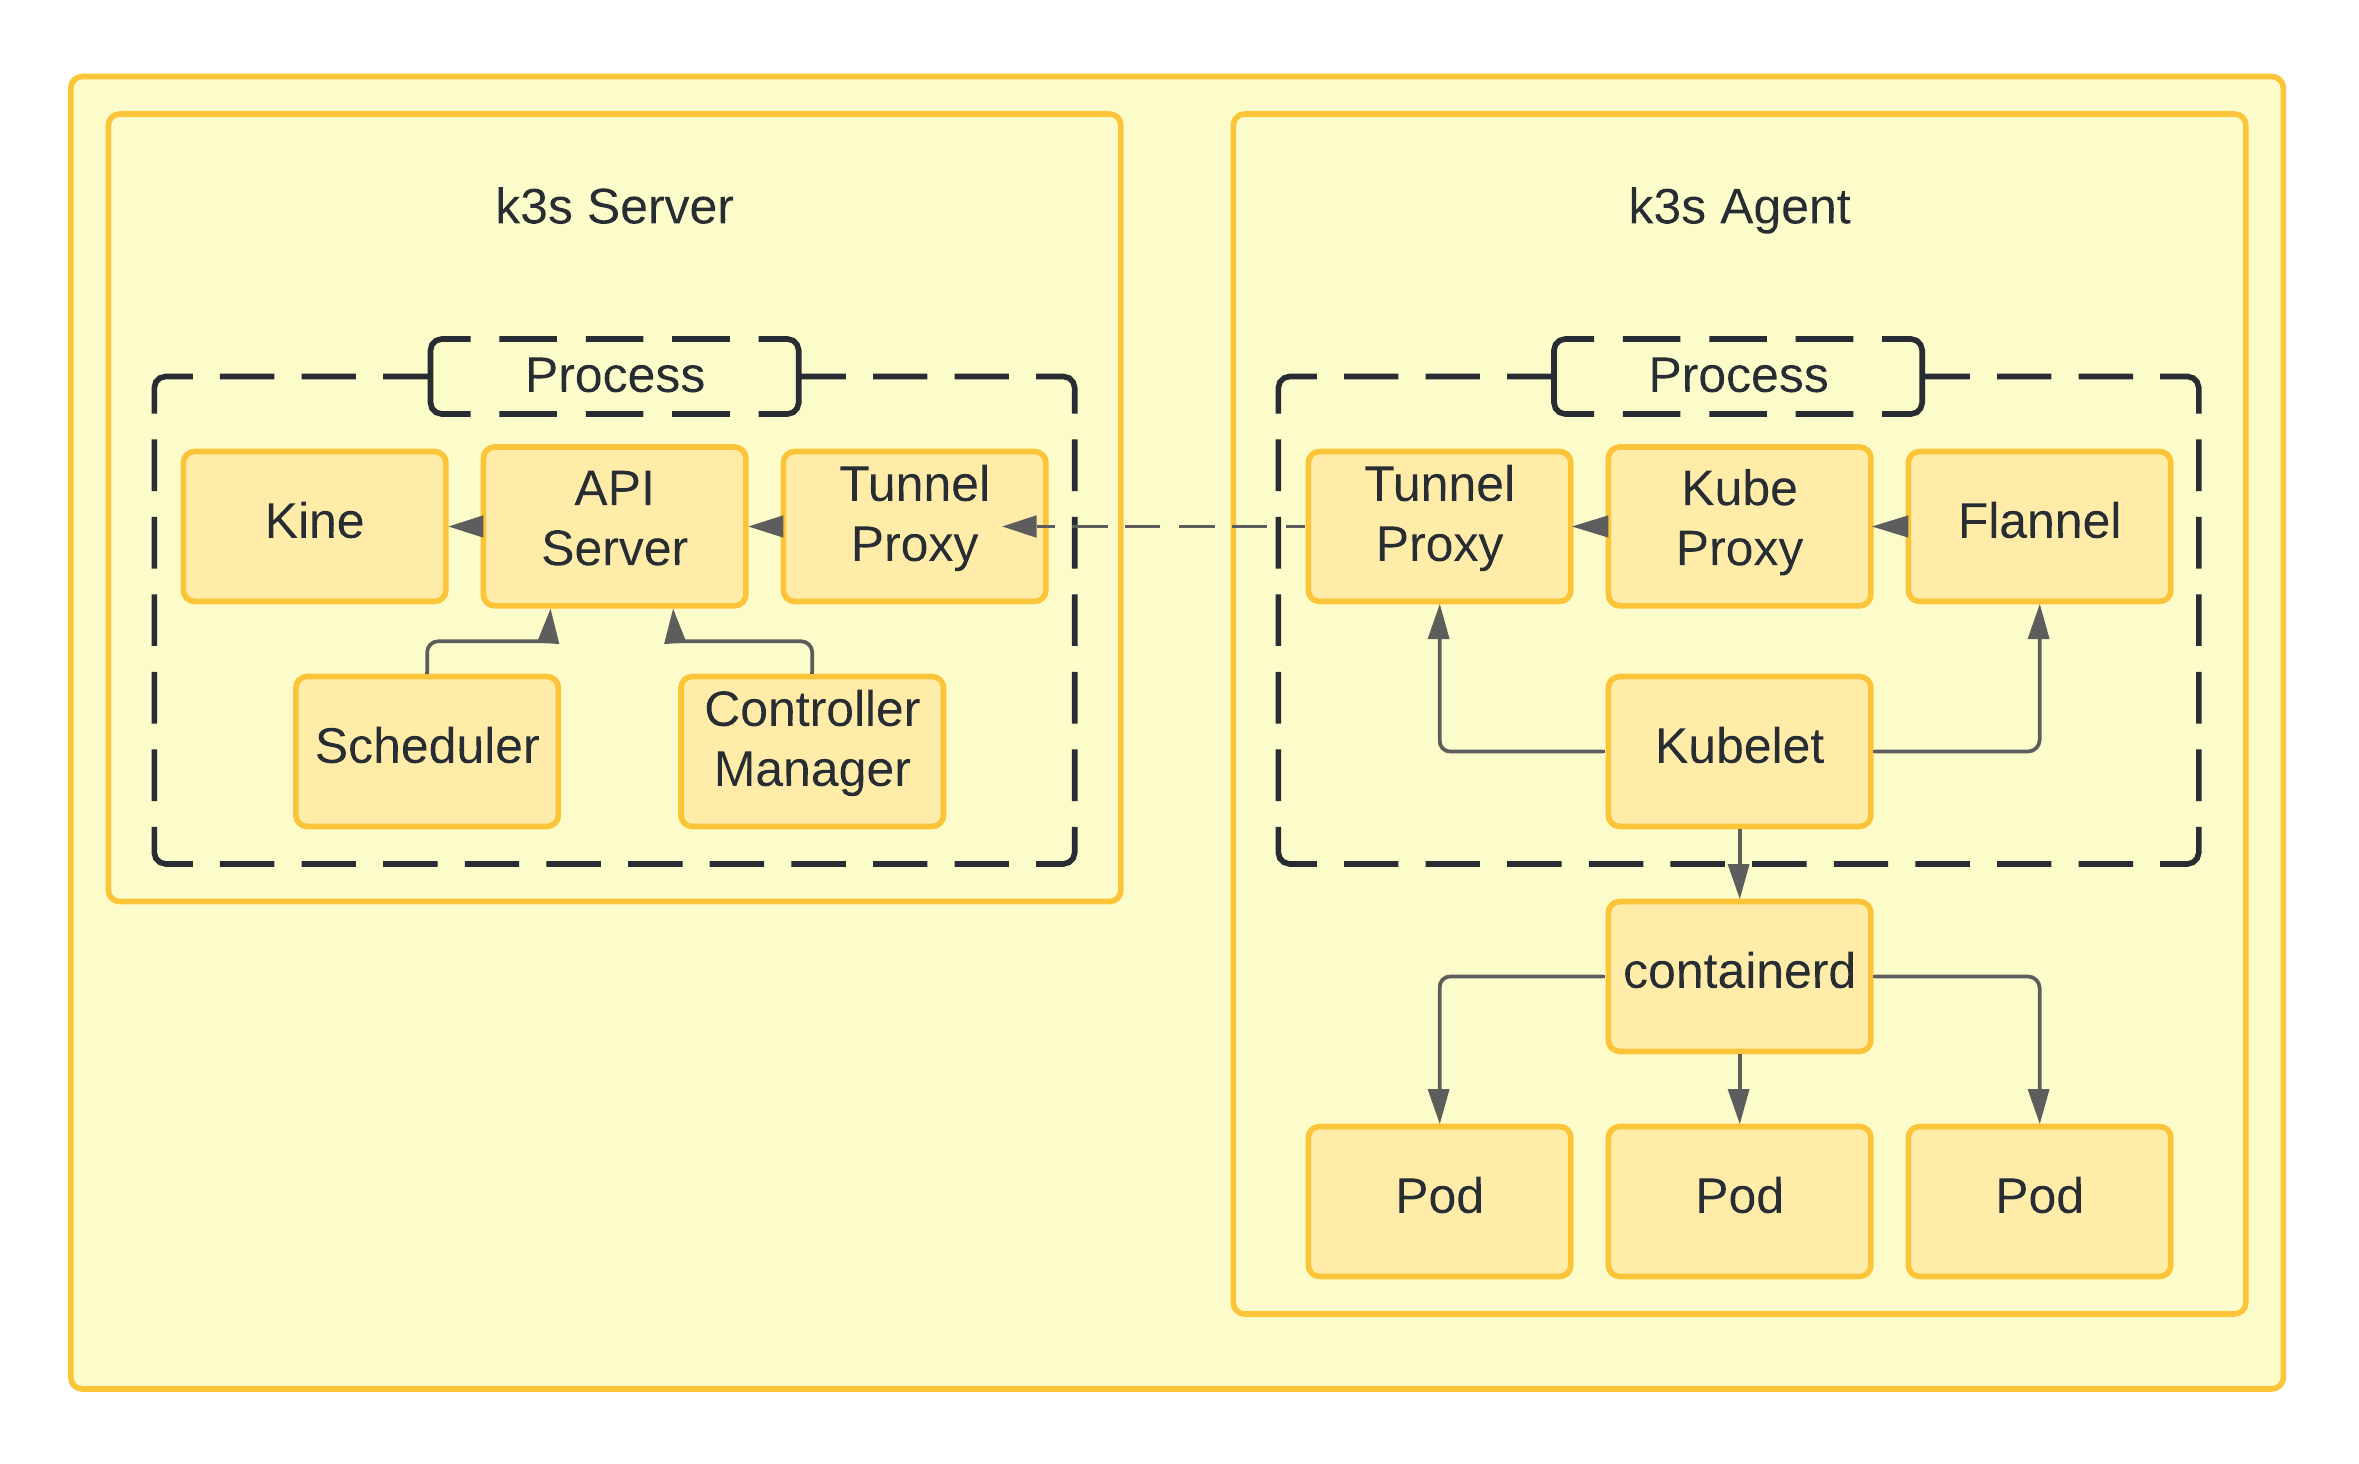
\includegraphics[width=1.0\columnwidth]{images/K3sArchitektur.png}
  \caption{K3s Architektur in Anlehnung an \cite{k3s}.}
  \label{fig:k3sarchitektur}
\end{figure}

\subsubsection{Besonderheiten}
Die Abbildung \ref{fig:k3sarchitektur} zeigt die Architektur von k3s auf. Das Kubernetes-Äquivalent zur Control Plane und Node
sind Server und Agent. Eine Besonderheit hiervon ist, dass Server parallel einen Agent-Prozess auf dem selben Knoten starten und
somit Arbeitslasten mithilfe von Kubelet ausführen \cite{k3sServerAgent}. Weiterhin wird, im Gegensatz zu Kubernetes, containerd weiterhin unterstüzt und
kommt mit Kubelet vorinstalliert \cite{k3s}. Zwei weitere Unterschiede werden näher erläutert:

\textbf{Kine}
das Akronym steht für \glqq Kine is not etcd\grqq{} und ist eine Abstraktionsschicht für die etcd \acs{api} und übersetzt die Aufrufe von Kubernetes in sqlite, Postgress, Mysql und dqlite \cite{k3sgit}.
Dadurch kann der Backend Speicher des Clusters durch die oben genannten Datenbanksysteme ersetzt werden.

\textbf{Flannel}
ist ein überlagerndes Netzwerkmodell in k3s und ermöglicht IPv4 Netzwerke innerhalb eines Clusters mit mehreren Knoten.
Dazu wird eine einzelne Binärdatei gestartet, welche Agents auf Hostssystemen startet. Dieser alloziert Subnetze in einem vorkonfigurierten Adressraum.
Das Modell ist dabei für die Übertragungsart des Datenverkehrs zwischen unterschiedlichen Knotenpunkten zuständig.
Die Speicherung der Netzwerkkonfiguration erfolgt über etcd oder der Kubernetes-\acs{api} \cite{flannel}.


\subsection{Rancher}
In diesem Unterabschnitt wird die Open-Source-Lösung Rancher von dem gleichnamigen Unternehmen zur Orchestierung von Kubernetes Clustern näher behandelt.
Sie ermöglicht das Verwalten von Kubernetes-Clustern auf der eigenen Infrastruktur, sowohl vor Ort als auch in der Cloud.
Die Bereitstellung von Clustern mittels Rancher ist Cloud-Anbieter unabhängig,
weshalb Cluster in der Praxis mit derselben Rancher Instanz auf \acs{aws}, Azure oder anderen Cloud-Anbietern betreut werden können \cite{rancher}.

Die Rancher-Benutzeroberfläche vereinfacht das Steuern von Arbeitslasten, auf einer zentralen administrativen Instanz, welche gleichzeitig Authentifizierung und Rechteverteilung von Benutzern anbietet.
Das grundsätzliche Verwalten von Arbeitslasten verlangt kein tiefgründiges Wissen bezüglich Kubernetes-Konzepte. 
Die mitgelieferten Tools ermöglichen die Auslieferung und Verbindung von Kubernetes-Objekten und abstrahieren die Komplexität, die für die Betreuung eines solchen Systems notwendig sind \cite{rancher,AzureKubernetesService}.

Für komplexere Konfigurationen kann über die Oberfläche ein Terminal mit Kubectl aufgerufen werden.
Wie auch in Kubernetes ist der Zugang auf ein Kubernetes-Cluster von einer lokalen Entwicklungsumgebung mit einer kubeconfig-Datei möglich, diese beeinhaltet die Adresse zum Rancher-Server, Nutzerrechte und Zertifizierungszeichen \cite{rancherKubeconfig}.

\begin{figure}[!htb]
  \centering
  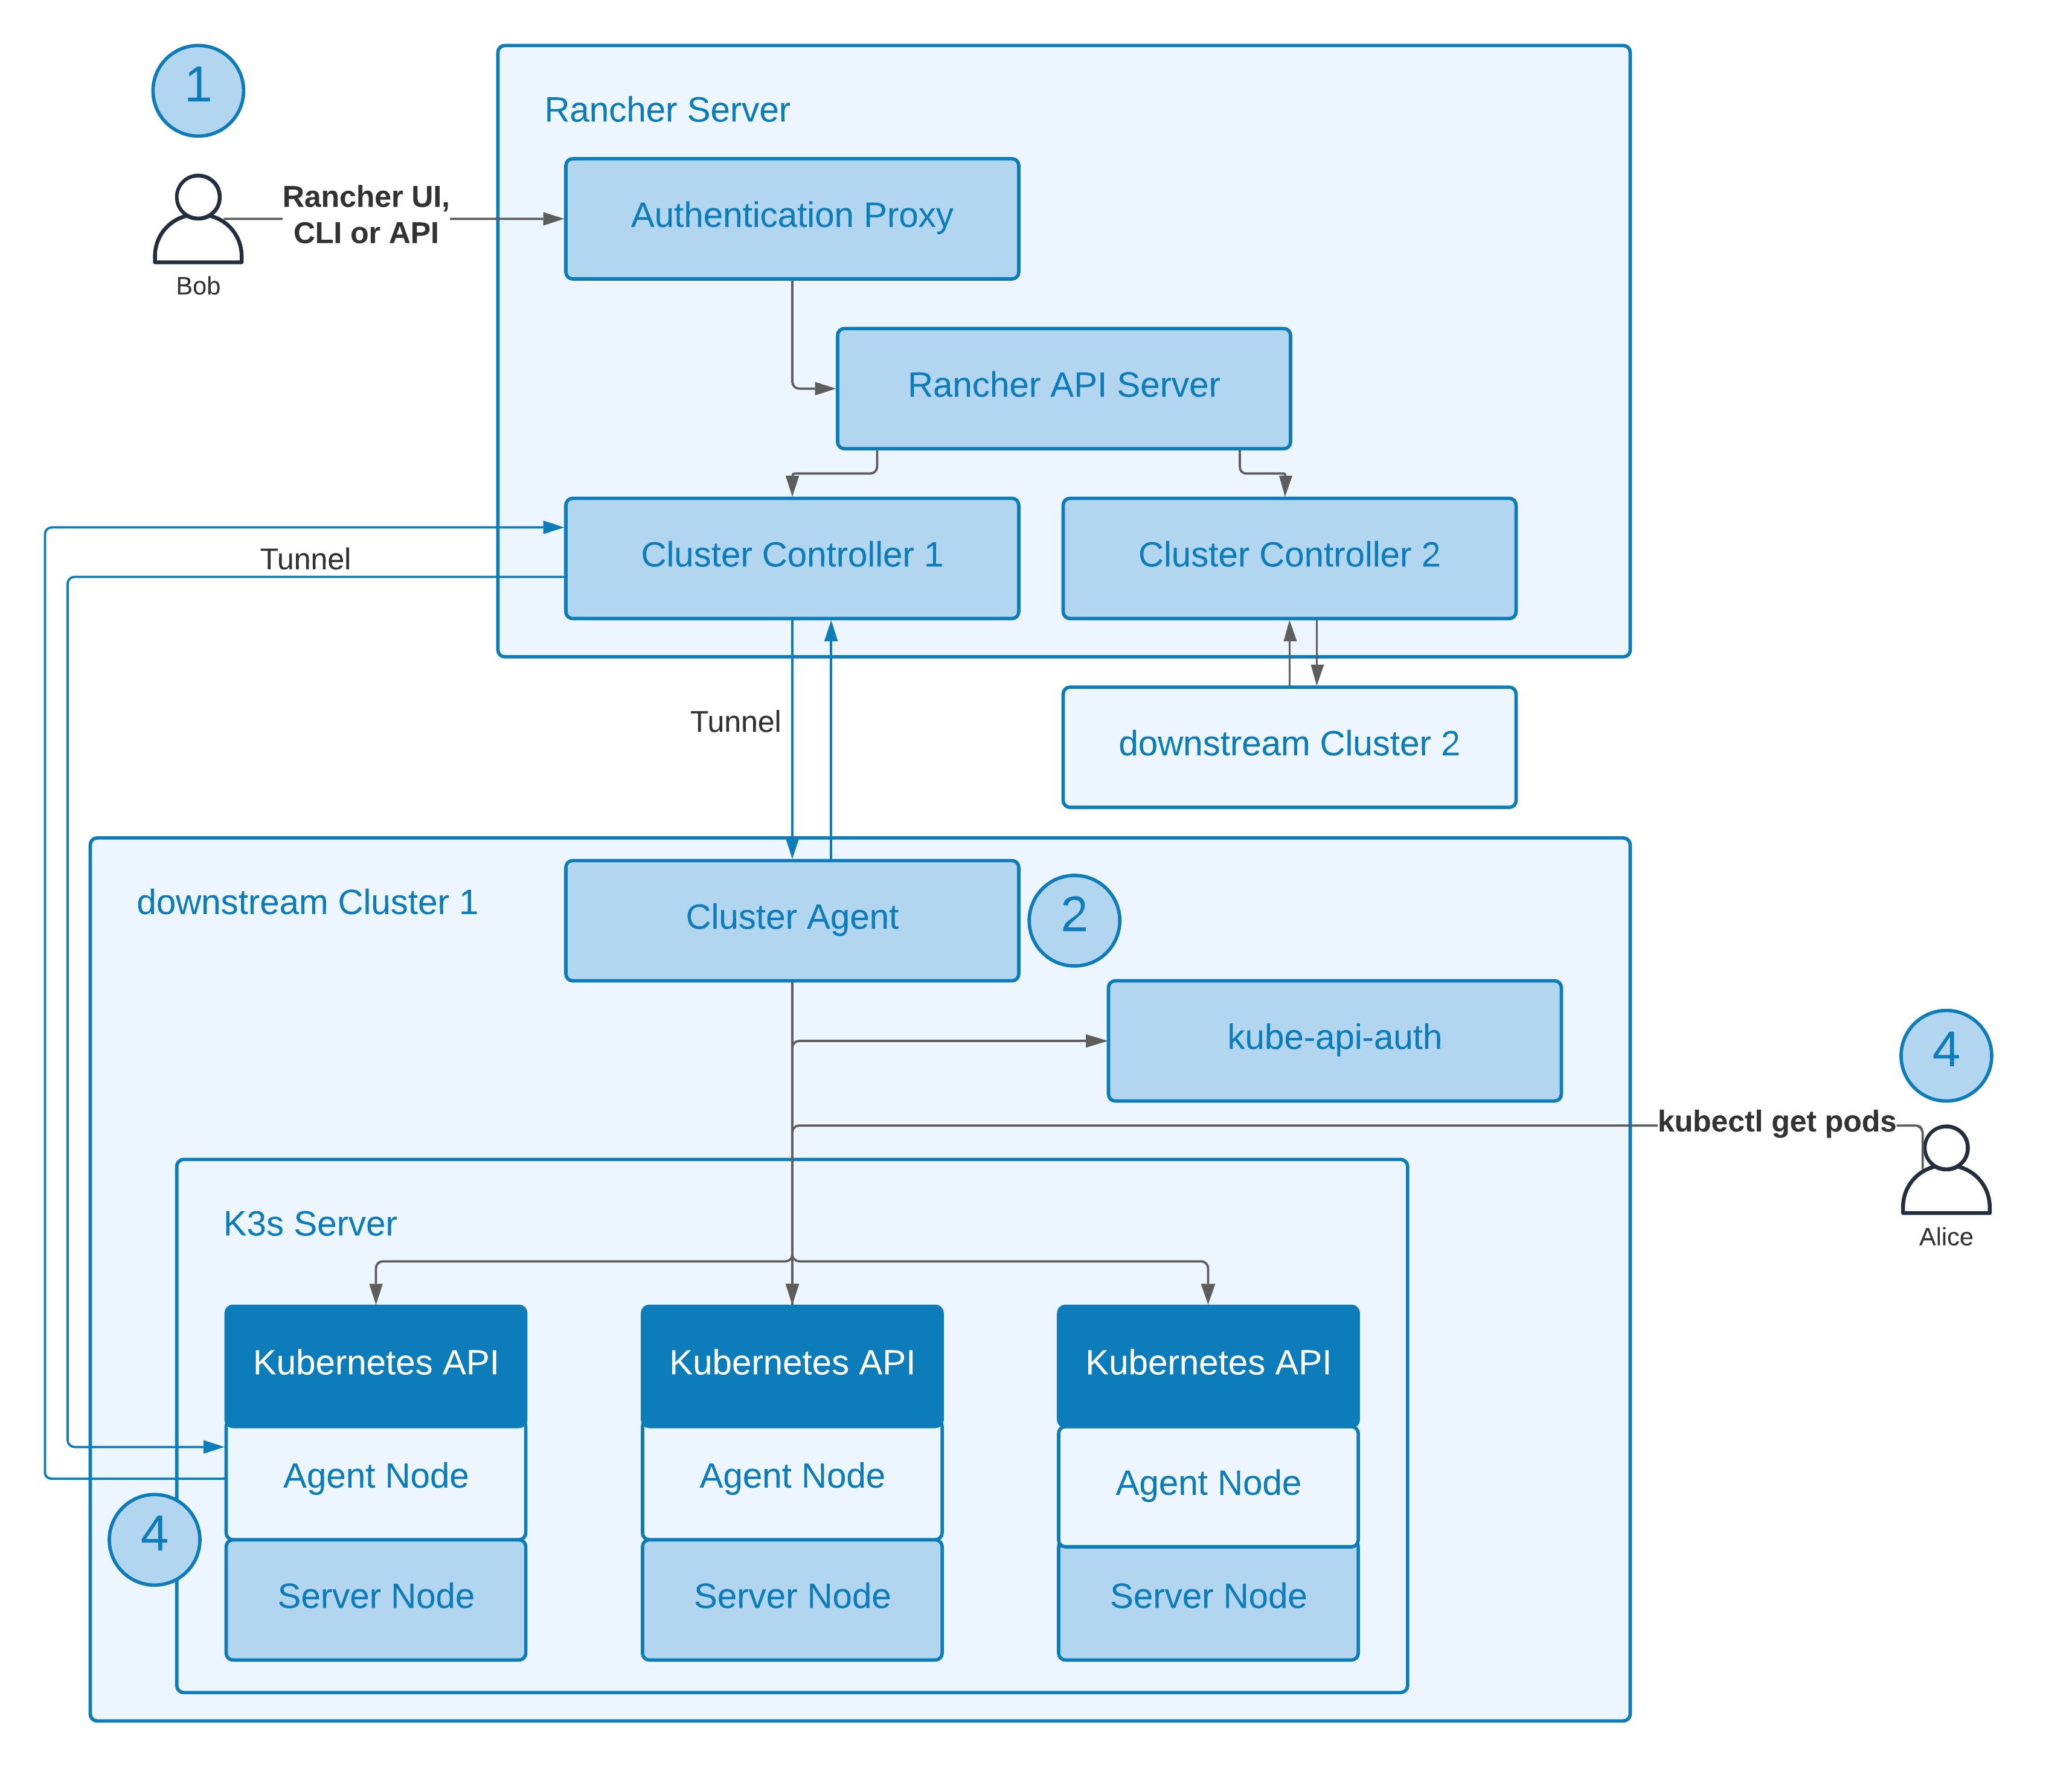
\includegraphics[width=0.8\columnwidth]{images/RancherArchitekturClusterController.png}
  \caption{Rancher Server Kommunikation mit einem downstream k3s Cluster, überarbeitete Abbildung von \cite{rancherArchitecture}. (Im Sinne der späteren Architektur nachgebildet)}
  \label{fig:rancherarchitektur}
\end{figure}

Die Abbildung \ref{fig:rancherarchitektur} zeigt den Vorgang von zwei Benutzern, 
die auf ein von Rancher verwaltetes downstream-k3s-Cluster\footnote{Die offiziele Bezeichnung für ein Kubernetes-Cluster unter Rancher ist \textbf{downstream Cluster} \cite{rancherArchitectureRecommendations}} zugreifen.
Die nachfolgende Beschreibung aus der Dokumentation gibt die einzelnen Schritte mit der in der Abbildung nummerierten Posten wieder \cite{rancherArchitecture}.


\begin{enumerate}
\item Zuerst authentifiziert sich Bob mit seinen Benutzerdaten bei dem Authentifizie\-rungs-Proxy an seinem Rancher-Server.
Dieser Proxy leitet den Aufruf über eine Kommandozeile oder der Rancher-Benutzeroberfläche zu der ausgewählten downstream-Cluster-Instanz weiter und führt diese aus.
Dafür wird vor dem Weiterleiten des Aufrufs der angemessene Kubernetes-Impersonation-Header gesetzt, 
welcher sich als Service-Account der Rancher-Instanz ausgibt.   
\item Die Übertragung des Aufrufs erfolgt über einen Cluster-Controller auf dem Rancher-Server
und dem parallel laufenden Cluster-Agent des downstream-Clusters. Der Controller ist für die Überwachung, Veränderung
und Konfiguration von Zuständen auf dem laufenden Cluster zuständig. 
\item Wenn der Cluster-Agent nicht erreichbar ist,
werden die Aufrufe an den Node-Agent\footnote{Ein Rancher-DaemonSet zur Interaktion mit Nodes. 
Nicht zu verwechseln mit dem Node-Agent von k3s \cite{rancherAgents}. } überreicht, welcher standardmäßig auf jedem downstream-Cluster läuft.
\item Zuletzt hat auch die Benutzerin Alice die Möglichkeit, sich über einen autorisierten Cluster-Endpunkt zu verbinden.
Denn jeder downstream-Cluster verfügt über eine Kubeconfig, welche den Zugang ohne Authentifizierungs-Proxy erlaubt.
Durch den Microservice kube-api-auth wird eine Kommunikation über einen Web-Hook realisiert, der die Verbindung
zwischen Alice und dem downstream-Cluster aufbaut. 
Dies ermöglicht die Verwendung von Befehlszeilentools, wie Kubectl und Helm.
\end{enumerate}

%\section{Distributed Clouds}
%\subsection{Edge Computing}
\subsection{Hybrid Cloud}
Eine Hybrid-Cloud ist eine Kombination aus öffentlichen und privaten Cloud-Diensten, die auf einer einzigen Infrastruktur laufen.
Dies ermöglicht die flexible Orchestrierung von Anwendungen auf Hostssystemen vor Ort oder in der Cloud \cite{ibmHybrid}.

Der Schwerpunkt solcher Hybrid-Clouds liegt dabei bei der Portierbarkeit der Arbeitslasten auf allen Cloud-Umgebungen.
Dafür ist die Aufbereitung oder Entwicklung alter oder neuer Anwendungen für cloudnative Technologien nötig; mehr dazu im Abschnitt \ref{Microservice} zu Microservices.
Private-Clouds können auch von Drittanbietern, durch externe Rechnzentren, als Enterprise Modell angeboten werden. Dabei ist die Nutzung eines einzigen Betriebssystems ratsam, um Abhängigkeiten bei der Automatisierung von cloud-nativen Anwendungen zu verhindern.
Die Verwaltung erfolgt, dabei mit einer Container-Orchestierungsplattform, wie Kubernetes und ermöglicht die nahtlose Implementierung von Cloud-Umgebungen \cite{ibmHybrid}.

\section{Microservice}\label{Microservice}
Im Folgenden wird der Microservice Architektur-Stil und dessen Eigenschaften näher erläutert.
Als Hauptquelle dient der häufig zitierte Artikel \cite{FowlerMicroservice} von Fowler und Lewis.

\subsection{Begriffserklärung}
Fowler und Lewis beschreiben den Microservice-Architektur-Stil als Entwicklung einer einzigen Anwendung, die aus einer Reihe unabhängiger Dienste besteht. 
Die Kommunikation der einzelnen Dienste untereinander wird häufig durch \acs{api}-Aufrufe über \acs{http} realisiert. 
Diese Dienste sind vollautomatisch auszuliefern und orientieren sich bei der Entwicklung um Business-Capabilities\footnote{Business-capability bezeichnet ein Konzept, das aus Sicht der Geschäftsarchitektur modelliert wird \cite{MicroservicePattern}}. 
Zusammenhängende Dienste werden minimal zentral gehalten und können in unterschiedlichen Programmiersprachen oder Technologien realisiert werden \cite{FowlerMicroservice}.

\begin{figure}[!htb]
  \centering
  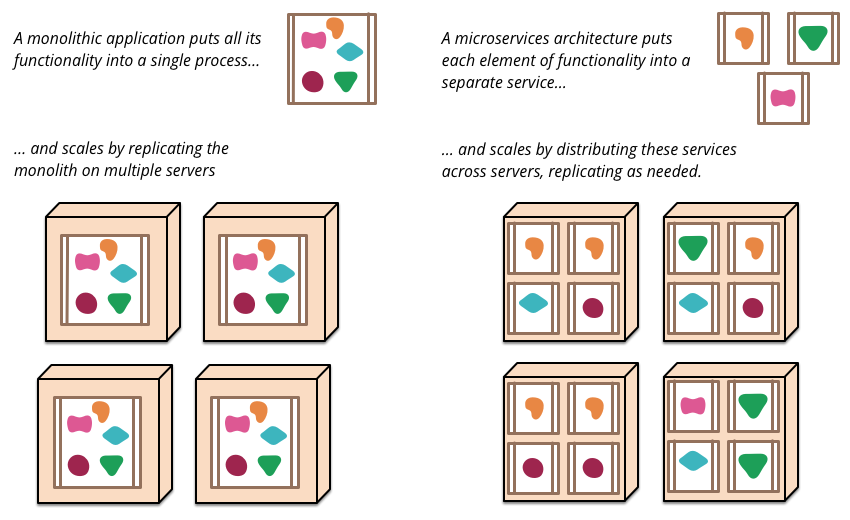
\includegraphics[width=0.8\columnwidth]{images/MonolithsAndMicroservices.png}
  \caption{Gegenüberstellung von Monolithen und Microservices \cite{FowlerMicroservice}}
  \label{fig:monlithmicroservice}
\end{figure}

Sinnvoll ist es hierbei, den Vergleich zu monolithischer Softwareentwicklung zu ziehen. 
Ein Monolith folgt hierbei der Grundprämisse mittels, der verwendeten Programmiersprache die Anwendung in einzelne Klassen, Funktionen und Namensräume aufzuteilen. 
Dieser Ansatz ist gängig und erfolgsversprechend. 
Jedoch argumentieren Fowler und Lewis, dass mit dem Zuwachs an Cloud-Technologien dieser Ansatz immer frustrierender für Entwickler ist, denn bereits kleine Änderungen an einem Modul benötigen einen neuen Software-Build und Auslieferungsprozess. 
Weiterhin merken Fowler und Lewis an, dass die Skalierbarkeit einer solchen Architektur mehr Ressourcen erfordert, da nicht einzelne Teile der Anwendung repliziert werden, sondern der vollständige Monolith (vgl. Abbildung~\ref{fig:monlithmicroservice}).
Die Verwendung von einzelnen Diensten würde dieser Problematik entgegentreten und es Entwicklerteams ermöglichen einzelne Softwarekomponenten zu verwalten und gegebenenfalls in einer anderen Programmiersprache zu verwirklichen \cite{FowlerMicroservice}.

\subsection{Charakteristiken}

Eine Microservice-Architektur prägt sich durch bestimmte Charakteristika aus. 
Die Architektur muss nicht zwingend alle in diesem Abschnitt beschriebenen Eigenschaften erfüllen. 
Jedoch sollte ein Großteil der Konzepte in einer Microservice-Architektur auffindbar sein \cite{FowlerMicroservice}. 
Die folgenden Unterabschnitte erläutern diese Charakteristika etwas näher.

\subsubsection{Komponententrennung durch Dienste}\label{TrennungdurchDienste}
Fowler definiert Komponenten einer Software wie folgt: \begin{quote}\glqq Eine Komponente ist eine Softwareeinheit, die unabhängig austauschbar und erweiterbar ist.\grqq{} \cite{FowlerSoftwareComponent} \end{quote}

Dienste einer Microservice-Architektur stellen Softwarekomponenten dar, die mittels Web-Service-Anfragen oder Remote-Procedure-Calls\footnote{Remote-Procedure-Calls bezeichnet die Ausführung eines lokalen Aufrufs auf einem anderen Dienst \cite{BuildingMicroservicesNewmanChapter5}.} interagieren.
Bibliotheken hingegen beschreiben einen Verbund aus mehreren Komponenten, die lokale Funktionsaufrufe nutzen. 
Der resultierende Vorteil ist, dass Dienste unabhängig voneinander verändert und ausgeliefert werden können. 
Denn bei Prozessen mit mehreren eingebundenen Bibliotheken, muss die gesamte Anwendung neu ausgeliefert werden \cite{FowlerMicroservice}. 

Dadurch wird der Fokus auf die Entwicklung von unabhängigen Diensten umso wichtiger, da die Veränderung an kooperierenden Schnittstellen zum Ausfall anderer Dienste führt. 
Um dem entgegenzuwirken, müssen Schnittstellen gut koordiniert werden und eine starke Kohäsion gewährleisten. Service Contracts\footnote{Service Contracts bezeichnen die Vereinbarung zwischen zwei Diensten, darin werden die Übertragungsformate von Daten festgelegt \cite{microservicesvssoa}.} der jeweiligen Dienste müssen sinnvoll gestaltet werden. 
Weiterhin müssen Schnittstellen grobkörniger entworfen werden, um den höheren Ressourcenverbrauch der lokalen Variante auszugleichen \cite{FowlerMicroservice, BuildingMicroservicesNewman}. 

Ein Dienst kann jedoch aus mehreren Prozessen bestehen. Ein Beispiel wäre ein Anwendungsprozess mit einer Datenbank, die nur von dieser Anwendung genutzt wird \cite{FowlerMicroservice, BuildingMicroservicesNewman}.

\subsubsection{Strukturierung nach Business-Capabilities}
Bei der Entwicklung von großen Anwendungen werden Teams oft nach technologischen Schichten getrennt. 
Es werden Teams aus Benutzeroberflächen-, Anwendungs- und Datenbankentwicklern gebildet. 
Die Entwicklung einer Microservice-Architektur bedarf jedoch eine Organisierung um die Business-Capabilities. 
Entwickler arbeiten funktionsübergreifend in allen Bereichen der Softwareentwicklung und bringen vielfältige Kompetenzen mit.
Der Grund dafür ist, dass bei Konstellationen mit einseitiger Softwarekompetenz, kleinste Änderungen zu teamübergreifenden Projekten und den damit verbundenen Kosten führt.
Effiziente Entwickler werden sich immer für den Weg des geringsten Widerstands entscheiden und ihre Logik dort implementieren, zu der das Team Zugang hat \cite{FowlerMicroservice}.

\subsubsection{Produkte nicht Projekte}
Microservice-Entwicklungen tendieren dazu, den kompletten Lebenszyklus einer Software zu begleiten. 
Der inspirierende Leitspruch bei Amazon dazu ist \begin{quote}
  \glqq  you build it, you run it \grqq{} \cite{amazon}.\end{quote} 
Dem Gedanken nach übernimmt das Entwicklungsteam die vollständige Produktion der Software und übergibt diese nicht an ein Wartungsteam. 
Dadurch stehen die Entwickler im direkten Kontakt mit dem Endnutzer und erfahren wie sich die Software im Betrieb verhält, da diese auch Zuständigkeiten des Supports übernehmen \cite{FowlerMicroservice}.

\subsubsection{Intelligente Endpunkte statt komplexer Infrastruktur}
Die Kommunikation von Diensten über Endpunkte soll so weit wie möglich entkoppelt und kohäsiv sein.  
Anwendungen im Microservice-Stil enthalten ihre eigene Logik und agieren als Filter für das Empfangen, Verarbeiten und Beantworten einer Anfrage. 
Die Umsetzung erfolgt dabei mit \acs{rest}ful-Protokollen für die Kommunikation über \acs{http} oder der leichtgewichtigen Kommunikation mit Messaging\footnote{Kommunikation über Binäre Protokolle wie Protocol-Buffers \cite{ProtoBuf}.}.
Ein weiterer Ansatz ist der Nachrichtenaustausch über leichtgewichtige Bussysteme.
Die gewählte Infrastruktur muss hier nicht mehr als einen rudimentären Informationsaustausch gewährleisten. 
Die Dienste sind so konzipiert, den größten Mehrwert über Endpunkte zu erreichen und Redundanz beim Nachrichtenaustausch zu vermeiden.

\subsubsection{Dezentrale-Governance}
Die Dezentralisierung einer Anwendung in Softwarekomponenten ermöglicht den Einsatz von unterschiedlichen Technologien. 
Da die einzelnen Anwendungskomponenten über Endpunkte kommunizieren, ist die Wahl der Programmiersprache weniger relevant als bei einer monolithischen Architektur. 
Entwicklerteams gewinnen so an Handlungsspielraum und können bessere Werkzeuge für spezifische Probleme verwenden \cite{FowlerMicroservice}.

\subsubsection{Dezentrales Datenmanagement}
Die Dezentralisierung von Daten geschieht auf höchster Ebene und abstrahiert diese für kontextbasierende Modelle. 
Die Integration solcher Modelle wird durch die unterschiedliche Auffassung verschiedener System erschwert. 
Dabei besteht die Gefahr das Abteilungen innerhalb eines Unternehmens Attribute unterschiedlich interpretiert und zu Inkonsistenz in Datensätze führt.
Eine Anwendung mit getrennten Softwarekomponenten erhöht diese Komplexität weiter \cite{FowlerMicroservice}. 
Weshalb es sinnvoll ist, einen \glqq Bounded Context\grqq{} zu definieren, welcher zur Darstellung von Wechselwirkungen eines Modells innerhalb größerer Teams dient \cite{FowlerBoundedContext}. 

%\subsubsection{Automatisierung von Infrastruktur}
%Das testen, ausliefern und bereitstellen von Microservices erfolgt automatisch \cite{FowlerMicroservice}. 
%Dieses Thema fällt in den Bereich Continuous Delivery und wird in dieser Arbeit nicht weiter behandelt. 

\subsubsection{\glqq Design for failure\grqq{}}
Softwarekomponenten müssen den Ausfall von anderen Diensten tolerieren. 
Event-basierte Kommunikation führt oft zu Fehlverhalten und kann durch Überwachungstools präventiv verhindert werden \cite{FowlerMicroservice}. 
